\documentclass{beamer}
\usepackage[utf8]{inputenc}
\usepackage[T1]{fontenc}
\usepackage{graphicx}
\usepackage{multicol}
\graphicspath{{./images/}}

\usetheme{Arguelles}

\title{Using FPGAs to Perform Cryptanalytic Attacks on Random Number Generators}
\subtitle{}
\date{27/5/2021}
\author{Andreas Stocker}
\institute{University of Nicosia\par\email{andreas@stockers.org}}

\begin{document}

  \frame[plain]{\titlepage}
  

  \begin{frame}
    \frametitle{Abstract}
    \framesubtitle{The purpose of this paper}

    This paper combines two somewhat unrelated subjects, FPGAs and cryptanalysis.
    It provides background on both of these subjects and then culminates
    in an experiment that combines the two.
  \end{frame}

  \Section{FPGAs}

  \begin{frame}
    \frametitle{What are FPGAs?}


    \begin{multicols}{2}

    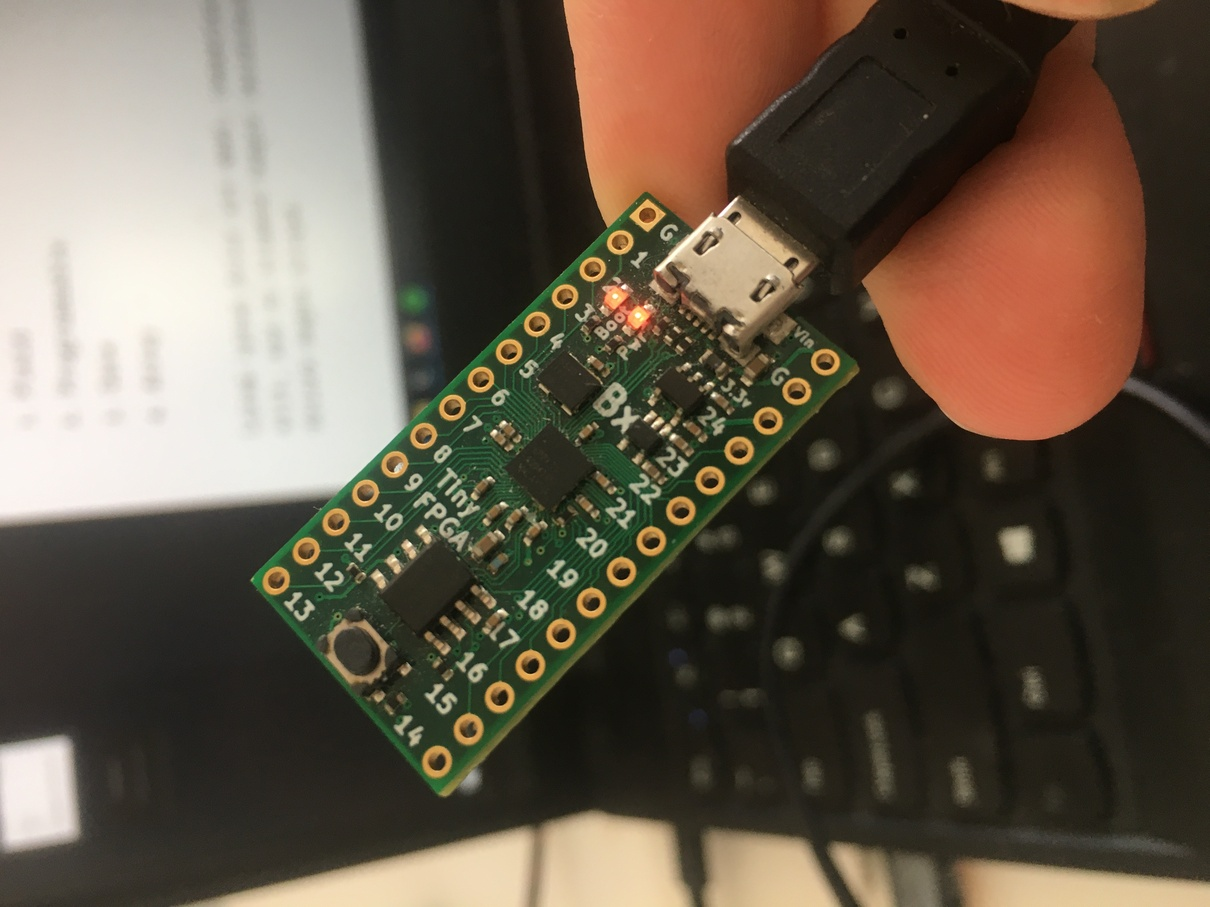
\includegraphics[scale=0.15,angle=-90]{tinyfpga-bx}
    
    \vfill
    
    \vspace*{\fill}
    
    \AlegreyaExtraBold FPGA \ttfamily stands for:
    \begin{enumerate}
      \item Field
      \item Programmable
      \item Gate
      \item Array
    \end{enumerate}
    
    \vspace*{\fill}

    \end{multicols}
    
  \end{frame}
  
  \begin{frame}
    \frametitle{FPGA Core Components}
    FPGAs are composed of the following \textit{core components}:
    \begin{itemize}
      \item Programmable Logic Blocks (PLBs)
      \item Specialized Logic Blocks
      \item Routing
      \item Clocks
    \end{itemize}
  \end{frame}
  
  \begin{frame}
    \frametitle{FPGAs verses ASICs}
    \framesubtitle{What are ASICs?}

    \textit{ASICs} are "Application Specific Integrated Circuits".

    \vfill

    CPUs for example are one of many types of ASICs.

    \vfill

    ASICs are produced through a silicon etching process that
    involves shining light through a mask and onto a photosensitive substance.

  \end{frame}
  
  \begin{frame}
    \frametitle{FPGAs verses ASICs}
    \framesubtitle{How do ASICs differ from FPGAs}

    Like the name suggests, FPGAs are \textit{field programmable}. \\
    This means the circuit of an FPGA can be quickly reconfigured.

    \vfill

    ASICs cannot be reconfigured and their circuit structure
    is set in stone from the time they were manufactured.

    \vfill

    Technically speaking, FPGAs themselves are a type of ASIC.

    \vfill

    There are numerous pros and cons that arise from these properties.

  \end{frame}

  
  \begin{frame}
    \frametitle{FPGAs verses ASICs}
    \framesubtitle{Where ASICs Shine}

    The static nature of ASICs brings a number of advantages.

    \vfill
    
    \begin{itemize}
      \item Cheaper to \textit{mass produce}
      \item More energy efficient
      \item Higher performance
      \item More compact
    \end{itemize}

  \end{frame}

  \begin{frame}
    \frametitle{FPGAs verses ASICs}
    \framesubtitle{Where FPGAs Shine}

    \AlegreyaSansMedium While ASICs have the upper hand in most categories, FPGA's have
    one essential advantage:

    \vfill
    
    \AlegreyaBlack It's far easier to modify an FPGA's design than an ASIC's.
    
    \vfill
      
    \AlegreyaSansMedium Developing and producing an ASIC design can cost \AlegreyaBlack
    millions of dollars. \\
    
    \vfill
    
    \AlegreyaSansMedium Producing a mask alone is extremely expensive. \\
    The designers cannot afford to make any mistakes. \\

  \end{frame}

  
  \begin{frame}
    \frametitle{FPGA Design Workflow}
    \framesubtitle{The Tools}

    Programming Languages:
    
    \begin{itemize}
      \item Verilog
      \item VHDL
    \end{itemize}

    \vfill

    Toolchains:
    
    \begin{itemize}
      \item Xillinx Proprietary Toolchain
      \item Intel (Altera) Proprietary Toolchain 
      \item Project Icestorm - Open Source
    \end{itemize}

    \vfill

    For this experiment, Verilog and the Icestorm toolchain were used.

  \end{frame}


  \begin{frame}
    \frametitle{FPGA Design Workflow}
    \framesubtitle{Simulation}

    Emulate an FPGA using a regular CPU

    \vfill

    \begin{itemize}
      \item Symbiyosys - evaluates Verilog
      \item Verilator - compiles Verilog to C++
        \begin{itemize}
          \item High performance
          \item Industry standard
          \item Sophisticated mock environment
        \end{itemize}
    \end{itemize}

    \vfill

    Upside: allows all state to be inspected

    \vfill

    Downside: can generate huge, untractable amounts of data


  \end{frame}



  \begin{frame}
    \frametitle{FPGA Design Workflow}
    \framesubtitle{Verification}

    Uses proofs to find possible invalid states.

    \vfill

    Upside: does not require developer to anticipate states

    \vfill

    Downside: can be complex and unintuitive to use


  \end{frame}

  \begin{frame}
    \frametitle{FPGA Design Workflow}
    \framesubtitle{Synthesis}

    Generate a design that a real FPGA can be programmed with. \\
    Then program the FPGA and run the design.

    \vfill

    Upside: shows whether the final design works in the field

    \vfill

    Downsides:\\ -- Internal state remains a black box\\
    -- Long turnaround time - can take minutes or hours

  \end{frame}

  \Section{Crypto}

  \begin{frame}
    \frametitle{Crypto History}

    Cryptography has been used since ancient times. \\
    Julius Caesar used encryption to communicate with allies.
    
    \vfill

    Crytographic and cryptanalytic machines became prominent in the 20th century.
    
    \vfill
    
    In WW2, the Enigma machine and the machines created to break it by Alan Turing
    are some of the most well known examples.

  \end{frame}

  \begin{frame}
    \frametitle{Random Number Generators}

    Generate a sequence of numbers that \textit{appear} to be random.

    \vfill

    RNGs need to have several attributes to be secure and work well:
    
    \begin{enumerate}
      \item Sufficient initital entropy
      \item Long period
      \item Even distribution of outputs
    \end{enumerate}
    
  \end{frame}
  
  \begin{frame}
    \frametitle{Linear Congruential Generators}

    Early implentations suffered from serious problems:
    \begin{enumerate}
        \item Get stuck at one value
        \item Short period
        \item Lack of even distribution
    \end{enumerate}

    \vfill

    Have three constant values that need to be tuned:
    \begin{enumerate}
        \item "m" - Modulus
        \item "a" - Multiplier
        \item "c" - Increment
    \end{enumerate}
    
    
  \end{frame}
  
  \begin{frame}
    \frametitle{Breaking Random Number Generators}

    Ways of attacking RNGs:
    \begin{enumerate}
        \item Recovering the internal state through another channel
        \item Brute force to recover seed and counter state
        \item "Backtracking" - obtaining previous states
    \end{enumerate}
    
  \end{frame}
  
  \begin{frame}
    \frametitle{Securing Random Number Generators}

    Ways of securing RNGs:
    \begin{enumerate}
        \item Getting initial entropy from an unpredictable source
        \item Hashing the outputs
        \item Restarting periodically
    \end{enumerate}
    
  \end{frame}

   
  \ThankYou
  \begin{frame}[plain,standout]
    In combination with \textit{plain},\par
    it makes a nice thank-you slide!

    \vfill{Generated using \textit{Beamer} and the \textit{Arguelles} Theme}
  \end{frame}

\end{document}
